\documentclass[pdflatex,sn-basic,Numbered]{sn-jnl}

%%%% Standard Packages
\usepackage{graphicx}
\usepackage{amsmath,amssymb,amsfonts}
\usepackage{amsthm}
%% Standard Springer Nature Packages
\usepackage{multirow}
\usepackage{mathrsfs}
\usepackage[title]{appendix}
\usepackage{manyfoot}
\usepackage{booktabs}
\usepackage{textcomp}
\usepackage{xcolor}
\usepackage{algorithmic}
\usepackage{algorithm}
\usepackage{tikz}
\usetikzlibrary{shapes.geometric, arrows, positioning}

%% Restore standard LaTeX table float to prevent conflict between resizebox and sn-jnl threeparttable
\makeatletter
\let\table\tableorg
\let\endtable\endtableorg
\makeatother

\raggedbottom

\begin{document}

\title[FinRisk-Evo: Temporal Corporate Risk-Drift Detection]{FinRisk-Evo: Temporal Corporate Risk-Drift Detection from Annual Report Disclosures}

\author*[1]{\fnm{Megh} \sur{Doshi}}\email{megh.doshi23@spit.ac.in}

\author[1]{\fnm{Shrey} \sur{Dedhia}}\email{shrey.dedhia23@spit.ac.in}

\author[1]{\fnm{Dhruv} \sur{Shah}}\email{dhruv.shah23@spit.ac.in}

\author[1]{\pfx{Dr.} \fnm{Pramod} \sur{Bide}}\email{pramod\_bide@spit.ac.in}

\affil*[1]{\orgdiv{Department of Computer Engineering}, \orgname{Sardar Patel Institute of Technology}, \orgaddress{\city{Mumbai}, \postcode{400058}, \state{Maharashtra}, \country{India}}}

\abstract{Corporate annual reports provide longitudinal disclosures about financial, operational, regulatory, and strategic risks, but comparing these documents across reporting periods is difficult because of layout noise, paraphrasing, numerical changes, and imperfect paragraph alignment. This paper presents FinRisk-Evo, a prototype document-intelligence pipeline for retrieving and comparing risk-related passages across annual reports. The codebase contains PDF block filtering, a Neural Variational Document Model (NVDM) for latent representations, a TNCRM-style masked-language-model training procedure, vector retrieval with cross-encoder re-ranking, and a temporal transition component that produces a heuristic risk-drift score with an uncertainty proxy. We describe the architecture and implementation and examine the available report artifacts for Mahindra \& Mahindra, Reliance Industries, and Kotak Mahindra Bank. We also report an exploratory annotation exercise comprising 150 paragraph pairs, with 45 pairs independently labelled by all three annotators. On these shared pairs, 23 of 45 received unanimous labels; nominal Krippendorff's alpha was 0.250, indicating limited agreement and the need for clearer operational definitions before the labels can serve as a reliable benchmark. Unsupported multi-sector and forecasting claims from earlier drafts are omitted. The paper presents a prototype and exploratory case study, not a validated financial forecasting model, and identifies the additional ablations, independently labelled examples, and external validation needed for evaluation.}
\keywords{Intelligent information systems, Financial disclosure mining, Longitudinal document analysis, Information retrieval, Risk drift, Uncertainty estimation}

\maketitle

\section{Introduction}

\subsection{Background}
The digitization of financial reporting has produced rapidly increasing volumes of unstructured financial text, particularly annual reports (e.g., 10-K filings, integrated annual reports). These documents contain critical narrative disclosures about a company's operational liabilities, liquidity constraints, and strategic challenges \cite{campbell2014, kravet2013, linsley2006}. However, extracting comparable, risk-relevant passages from these documents can be labor-intensive and subjective, limiting the speed at which analysts can identify changes in disclosed exposures \cite{fisher2016}.

\subsection{Problem Statement}
Standard language models and traditional sentiment analysis face three limitations that are particularly relevant to longitudinal risk-drift analysis. First, \textit{scalar blindness} prevents models from distinguishing risk severity; we define this phenomenon as a numerical/scalar insensitivity where numerical values and trend verbs of vastly different magnitudes are mapped to near-identical sentiment vectors (e.g., treating a minor ``1\% decline'' and a large ``40\% plunge'' with equivalent negative polarity). Second, we refer to the loss of document-layout and positional context, which strips away paragraph positioning, confusing minor boilerplate notices with critical disclosures in the risk factor sections. Third, the lack of \textit{temporal logic} limits evaluations to static snapshots, failing to capture how a specific corporate risk (e.g., cybersecurity or labor shortages) evolves or drifts across consecutive fiscal years.

\subsection{Motivation}
Quantifying changes in disclosed financial risk is critical for risk management and asset pricing. Narrative disclosures may contain information relevant to risk monitoring that is not immediately visible in summary financial measures. Developing a system that filters out layout noise, understands numerical magnitudes, projects changes onto a continuous semantic axis, and provides uncertainty estimates allows investors to support early-warning risk monitoring and potentially inform investment decision-making.

\subsection{Key Contributions}
The main contributions of this work are summarized as follows:
\begin{itemize}
    \item We describe an end-to-end prototype for longitudinal paragraph retrieval and comparison across annual-report disclosures, combining document extraction, dual-stream representations, retrieval, re-ranking, and temporal scoring.
    \item We document a targeted numerical/change-related masking procedure (TNCRM) intended to increase the training emphasis on numeric tokens and magnitude expressions; its effectiveness is treated as an open empirical question rather than an established result.
    \item We specify the implementation of the Financial Risk Escalation Score (FRES), including its semantic-similarity gate and uncertainty-weighted score, and identify calibration choices that require independent validation.
    \item We provide an exploratory annotation exercise of 150 paragraph pairs, with 45 pairs assigned to all three annotators. The observed nominal Krippendorff's alpha of 0.250 is reported transparently and motivates further annotation-protocol refinement.
    \item We distinguish implemented components from claims that still require reproducible experiments, including comparative model performance, calibration, cross-sector generalization, and downstream financial-outcome prediction.
\end{itemize}

\subsection{Paper Structure}
The remainder of this paper is organized as follows: Section~2 reviews related work. Section~3 describes the system architecture and mathematical formulation. Section~4 documents the available data and exploratory annotation exercise. Section~5 discusses implications, limitations, and ethical considerations. Section~6 concludes and outlines future work.

\section{Literature Review \& Related Work}

We group prior studies into five primary areas: static financial sentiment analysis, variational topic modeling, recurrent neural trackers, generative financial language models, and longitudinal corporate disclosures.

\subsection{Thematic Grouping of Prior Work}
\subsubsection{Static Financial Sentiment Analysis}
Early methods used dictionaries like the Loughran-McDonald (LM) list \cite{loughran2011} to count negative words. Textual analysis of annual reports has long been established as a tool to measure disclosure quality \cite{li2010}, with machine-learning approaches also being used to discover and quantify risk types in 10-K textual disclosures \cite{bao2014}. Although tailored to finance, they ignore negations and contextual layout noise. Modern transformer architectures \cite{vaswani2017}, including finance-specific models such as FinBERT \cite{araci2019}, capture semantic context but exhibit scalar insensitivity on numeric variations. Probing studies confirm that standard pre-trained language models often show limited numeracy and scalar understanding \cite{wallace2019, thawani2021}. To resolve this, Jung and Jang \cite{jung2024} proposed Targeted Numerical Change-Related Masking (TNCRM) to bias masked language modeling toward numerical terms. However, their evaluation was limited to static sentence classification on news snippets.

\subsubsection{Variational Topic Modeling}
Topic modeling helps structure large corporate documents. Traditional Latent Dirichlet Allocation (LDA) models \cite{blei2003} suffer from poor topic coherence on short paragraphs. Miao et al. \cite{miao2016} introduced the Neural Variational Document Model (NVDM), utilizing Variational Autoencoders (VAEs) \cite{kingma2013} to learn continuous topic representations. Mir et al. \cite{mir2025} fused NVDM topics with sentiment weights for short text trends but did not apply them to multi-year reports or track temporal drifts.

\subsubsection{Recurrent Financial Trackers}
Recurrent architectures, including LSTMs \cite{hochreiter1997} and GRUs \cite{cho2014}, are commonly used to model sequential dependencies. Duan et al. \cite{duan2024} combined LDA topics, FinBERT, and BiGRUs (LFBP framework) for financial sentiment. However, their model was evaluated statically. Recurrent stock price models, such as the hybrid LSTM-GRU framework by Farhadi et al. \cite{farhadi2025} or the CNN-LSTM news fusion model by Moodi et al. \cite{moodi2024}, focus on stock market forecasting rather than identifying risk trajectories. Similarly, Biswas et al. \cite{biswas2025} and Chen et al. \cite{chen2024} utilized sequence architectures to model market indicators, neglecting narrative document drift.

\subsubsection{Generative Financial Language Models}
The advent of large language models (LLMs) has transformed computational finance. BloombergGPT \cite{wu2023bloomberggpt}, a 50-billion parameter decoder model pre-trained on a massive finance-specific corpus, demonstrated strong performance on financial tasks but remains closed-source and computationally prohibitive for local deployment. Similarly, the FinGPT framework \cite{yang2023fingpt, li2023fingpt} provides open-source instruction-tuned models and data-centric pipelines for financial text mining. However, these generative decoders can produce unsupported or hallucinated outputs, require significant computational overhead, and lack native mechanisms to estimate epistemic uncertainty (such as Monte Carlo dropout) necessary for risk-sensitive financial applications. Furthermore, long-document architectures like the Longformer \cite{beltagy2020longformer} are designed primarily for long-context encoding rather than explicit year-over-year paragraph alignment.

\subsubsection{Longitudinal Risk Disclosure and Textual Change Detection}
A separate thread of research investigates the evolution and change detection of corporate disclosures over time. Prior work has examined how financial-report text relates to risk-related outcomes and how mandatory risk-factor disclosures reflect firm risk \cite{kogan2009,campbell2014}. These studies motivate analysis of disclosure text but do not validate the present prototype or its FRES score. Dyer et al. \cite{dyer2017} systematically documented the structural evolution and growing length of 10-K disclosures over time, highlighting increasing boilerplate, redundancy, and reduced specificity in 10-K disclosures. Similarly, Filzen \cite{filzen2015} analyzed the information content of risk factor updates, showing that fresh disclosures represent timely responses to emerging operational shocks. Hassan et al. \cite{hassan2019} constructed firm-level political-risk measures using narrative pattern matching in quarterly transcripts, showing evidence that narrative risk tracking yields incremental signals over static financial accounting sheets. However, these classical studies relied on global document-similarity metrics (e.g., cosine similarity of TF-IDF vectors), simple pattern matching, or bag-of-words change indices. Recent works have attempted to model corporate report transitions using deeper neural encoders; for instance, Kravet and Muslu \cite{kravet2013} and Linsley and Shrives \cite{linsley2006} analyzed risk-disclosure increases qualitatively, noting that static disclosures often mask operational changes. Despite these insights, the reviewed financial-text literature provides limited evidence of integrated mechanisms for a granular paragraph-level longitudinal alignment, often conflating formatting variations with actual thematic shifts. FinRisk-Evo fills this gap by introducing a unified paragraph-level alignment and re-ranking framework combined with continuous semantic projection.

\subsection{Critical Analysis and Gaps}
Table \ref{tab:lit_survey} summarizes the methodology, datasets, and shortcomings of these core baselines. A key problem-level gap in existing literature is the lack of longitudinal tracking: much of the reviewed literature focuses primarily on static sentiment classification of isolated news snippets or global document similarity checks. Consequently, they are incapable of tracking the specific trajectory of corporate disclosures across consecutive years, ignore contextual document layouts, and suffer from numerical/scalar insensitivity.

\begin{table*}[t]
\centering
\caption{Literature survey of related methodologies and their scope}
\label{tab:lit_survey}
\resizebox{\textwidth}{!}{%
\begin{tabular}{lllll}
\toprule
Reference & Dataset & Methodology & Scope of reported work & Relevance to this study \\
\midrule
Duan et al. \cite{duan2024} & FiQA-SA, StockSen & LDA + FinBERT + BiGRU (LFBP) & Financial-text sentiment classification & Does not evaluate year-over-year annual-report paragraph alignment. \\
Mir et al. \cite{mir2025} & StockEmotions Dataset & VAE NVDM + FinBERT & Joint topic/emotion modeling in financial text & Different task and dataset from longitudinal disclosure comparison. \\
Jung \& Jang \cite{jung2024} & Financial PhraseBank & TNCRM Masking List (193 words) & Numerical-change-aware masking for financial language & Downstream value in this pipeline remains untested. \\
Farhadi et al. \cite{farhadi2025} & Tehran Stock Exchange & Hybrid LSTM-GRU technical model & Hybrid recurrent stock-price prediction & Focuses on price series rather than disclosure text. \\
Biswas et al. \cite{biswas2025} & Visa \& MasterCard (2008--2024) & Dilated TCN with self-attention & Temporal convolution for price and risk-metric forecasting & Uses market series rather than paragraph-level annual-report alignment. \\
BloombergGPT \cite{wu2023bloomberggpt} & Bloomberg Proprietary Dataset & 50B Decoder LLM & Finance-domain language model evaluated on finance tasks & Not a direct baseline for this prototype’s paragraph-pair task. \\
FinGPT \cite{yang2023fingpt} & Financial News \& Social Media & Instruction-tuned LLaMA-7B & Open financial-language-model framework & Not evaluated here on the same held-out paragraph pairs. \\
\bottomrule
\end{tabular}%
}
\end{table*}

\section{Methodology \& System Architecture}

\subsection{Overview}
The architecture of FinRisk-Evo is structured into five sequential layers: Geometric Layout Filtration, a VAE-based Context Engine (NVDM), a numerically-sensitive Precision Engine (TNCRM), a Recurrent Temporal Sequence Engine (BiGRU), and a Continuous Semantic Gating layer. The unified system flow is illustrated in Fig. \ref{fig:architecture}.

\begin{figure}[!t]
\centering
\resizebox{0.92\columnwidth}{!}{%
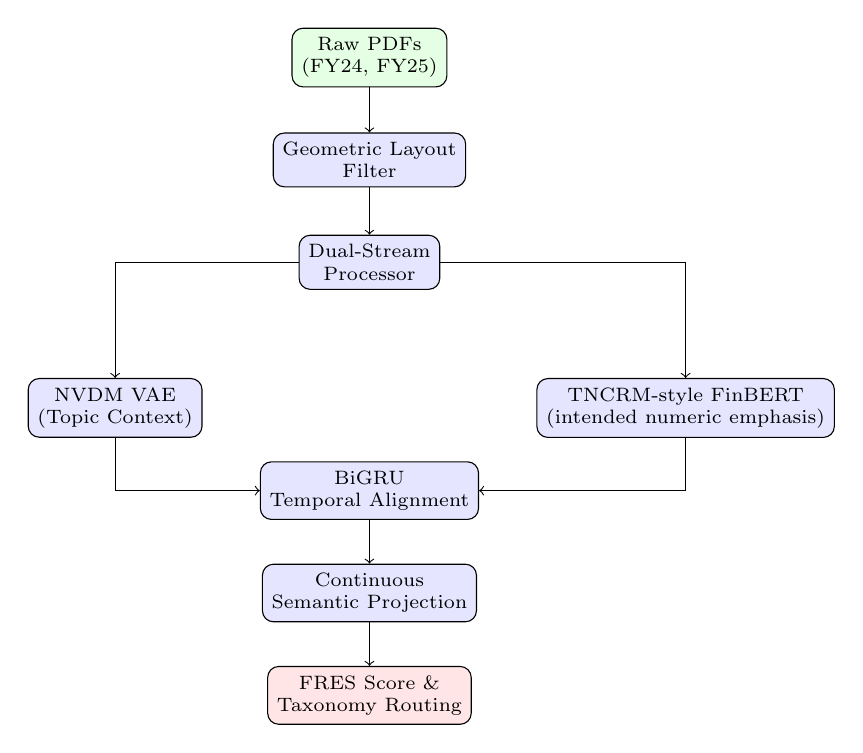
\begin{tikzpicture}[node distance=1.3cm, every node/.style={fill=blue!10, draw, rounded corners, font=\scriptsize, align=center}]
  \node (raw) [fill=green!10] {Raw PDFs\\(FY24, FY25)};
  \node (geo) [below of=raw] {Geometric Layout\\Filter};
  \node (dual) [below of=geo] {Dual-Stream\\Processor};
  \node (nvdm) [below left=of dual, xshift=-0.3cm, yshift=-0.2cm] {NVDM VAE\\(Topic Context)};
  \node (finbert) [below right=of dual, xshift=0.3cm, yshift=-0.2cm] {TNCRM-style FinBERT\\(intended numeric emphasis)};
  \node (align) [below of=dual, yshift=-1.6cm] {BiGRU\\Temporal Alignment};
  \node (proj) [below of=align] {Continuous\\Semantic Projection};
  \node (fres) [below of=proj, fill=red!10] {FRES Score \&\\Taxonomy Routing};
  
  \draw[->] (raw) -- (geo);
  \draw[->] (geo) -- (dual);
  \draw[->] (dual) -| (nvdm);
  \draw[->] (dual) -| (finbert);
  \draw[->] (nvdm) |- (align);
  \draw[->] (finbert) |- (align);
  \draw[->] (align) -- (proj);
  \draw[->] (proj) -- (fres);
\end{tikzpicture}%
}
\caption{System architecture of the FinRisk-Evo temporal risk modeling framework}
\label{fig:architecture}
\end{figure}
\subsection{Geometric Layout Filtration}
To remove running page headers, footers, and stamps, we process blocks using coordinate checking. Let the page height be $H$. For text block $b_i$ with coordinate bounds $(x_0, y_0, x_1, y_1)$ and text string $s_i$, we preserve the block if and only if it satisfies:
\begin{equation}
y_0 \ge 0.08 \times H \quad \text{and} \quad y_1 \le 0.92 \times H
\end{equation}
The supplied extractor implements fixed 8\% top and bottom page-margin rules and excludes text blocks of 12 words or fewer. The available artifacts do not document a separate validation corpus or independently labelled gold-standard set for estimating filter precision or recall. Let $N_{\text{noise}}$ represent a hypothetical manually labelled set of layout-noise blocks and $N_{\text{filtered}}$ the blocks discarded by the coordinate check. If a gold-standard set is collected in future work, noise recall can be defined as:
\begin{equation}
R_{\text{noise}} = \frac{|N_{\text{noise}} \cap N_{\text{filtered}}|}{|N_{\text{noise}}|}
\end{equation}
We discard blocks matching regular expressions for page indices (e.g., \verb|^\d+$|) or report headers, ensuring that boilerplate text does not corrupt the downstream embeddings.

\subsection{Context Engine: Neural Variational Document Model}
Paragraphs are converted to nonnegative word-count vectors $\mathbf{x} \in \mathbb{R}^{V}$, where $x_w$ represents the raw count of word $w$ in the paragraph. The encoder maps $\mathbf{x}$ to the mean vector $\boldsymbol{\mu} \in \mathbb{R}^{K}$ and log-variance vector (where $K=20$). In the implementation, the mean vector is used as the paragraph-level latent representation; it is not a normalized topic-probability distribution. The variational loss is the negative Evidence Lower Bound (ELBO):
\begin{equation}
\mathcal{L}_{\text{ELBO}}(\theta, \phi; \mathbf{x}) = -\mathbb{E}_{q_\phi(\mathbf{z}|\mathbf{x})}[\log p_\theta(\mathbf{x}|\mathbf{z})] + D_{\text{KL}}(q_\phi(\mathbf{z}|\mathbf{x}) \parallel p(\mathbf{z}))
\end{equation}
where the KL divergence is defined as:
\begin{equation}
D_{\text{KL}} = -\frac{1}{2} \sum_{j=1}^{K} \left( 1 + \log \sigma_j^2 - \mu_j^2 - \sigma_j^2 \right)
\end{equation}
Here, $\mu_j$ and $\sigma_j^2$ represent the variational parameters of topic $j$. The reconstruction log-likelihood is approximated as:
\begin{equation}
\log p_\theta(\mathbf{x}|\mathbf{z}) = \sum_{w \in \mathbf{x}} x_w \log \text{softmax}(\mathbf{R}\mathbf{z} + \mathbf{b})_w
\end{equation}
where $\mathbf{R} \in \mathbb{R}^{V \times K}$ is the decoding weight matrix mapping topics back to vocabulary terms, and $\mathbf{b}$ is the bias vector.

\subsection{Precision Engine: Custom TNCRM Masking Collator}
The supplied TNCRM training script accepts a text corpus and applies a custom masking distribution, but the available repository does not substantiate a 50,000-sentence, 14-company training corpus. We therefore document the masking procedure without claiming that corpus size or company count as a verified experimental fact. Let $\mathcal{T}_{\text{num}}$ be the set of numerical tokens, $\mathcal{T}_{\text{mag}}$ be magnitude words, and $\mathcal{T}_{\text{special}}$ be special formatting or padding tokens. The masking probability $P_{ij}$ assigned to token $t_{ij}$ is:
\begin{equation}
P_{ij} = \begin{cases} 
0.75, & t_{ij} \in \mathcal{T}_{\text{num}} \cup \mathcal{T}_{\text{mag}} \\
0.10, & t_{ij} \notin \mathcal{T}_{\text{num}} \cup \mathcal{T}_{\text{mag}} \\
0.00, & t_{ij} \in \mathcal{T}_{\text{special}}
\end{cases}
\end{equation}
We use a 75\% masking probability for numerical tokens to emphasize quantitative severity markers during MLM training. This encourages the model to represent quantitative severity markers more distinctly.

The supplied artifacts do not contain independently generated predictions or logs for a controlled numerical-sensitivity experiment. We therefore describe TNCRM as a proposed training intervention and do not claim that it improves embedding sensitivity until the base and post-trained checkpoints are evaluated on a frozen, reproducible test set.

\subsection{Evolution Engine: Pairwise Longitudinal Transition Modeling}
We stack the NVDM latent-mean vector $\boldsymbol{\mu}$ and FinBERT embedding $\mathbf{s}_{\text{CLS}}$ to construct paragraph vector $\mathbf{v} = [\boldsymbol{\mu}; \mathbf{s}_{\text{CLS}}] \in \mathbb{R}^{788}$. For each target paragraph, candidate baseline paragraphs are retrieved using \texttt{all-MiniLM-L6-v2} embeddings in ChromaDB (restricted to the baseline reporting period). The top-5 candidates are then reranked using a cross-encoder (\texttt{cross-encoder/}\allowbreak\texttt{ms-marco-MiniLM-L-6-v2}) to optimize contextual matching. The selected baseline-target pair is subsequently represented using the concatenated NVDM and FinBERT vectors $\mathbf{v}_{t-1}$ and $\mathbf{v}_t$, building on dual-encoder semantic retrieval \cite{reimers2019} and cross-encoder passage re-ranking \cite{nogueira2019} techniques. The sequential transition pair $\mathbf{S} = [\mathbf{v}_{t-1}, \mathbf{v}_t]$ is passed to a BiGRU-based pairwise transition model. Although the sequence length is restricted to $T=2$ consecutive reporting periods (baseline and target) representing a pairwise temporal transition, the recurrent cell architecture is utilized to learn non-linear sequential transition mappings (modeling $\mathbf{v}_{t-1} \rightarrow \mathbf{v}_t$) and directional dependencies, which is the implemented pairwise transition architecture; no controlled comparison against MLP or Transformer alternatives is available in the current artifacts. Under Monte Carlo dropout \cite{gal2016} ($N=10$ stochastic forward passes), we output the mean probability $\bar{p}_{\text{risk}}$ and standard deviation $\sigma_{\text{risk}}$ across the stochastic passes, where $\bar{p}_{\text{risk}} = \frac{1}{N} \sum_{i=1}^{N} \sigma(y_i)$ and $y_i$ represents the logit output at stochastic forward pass $i$. The uncertainty-derived confidence weight is:
\begin{equation}
W_{\text{conf}} = 1 - \sigma_{\text{risk}}
\end{equation}
where $\sigma_{\text{risk}}$ is the standard deviation representing the MC-dropout uncertainty estimate across predicted probabilities. The current repository artifacts do not contain a reproducible, independently labelled holdout set or saved predictions sufficient to calculate calibration metrics. We therefore do not report ECE or Brier scores. In this implementation, the standard deviation of ten stochastic predicted probabilities is used as a heuristic uncertainty proxy; the resulting confidence weight is not a validated calibration measure.

\subsection{Continuous Semantic Projection and FRES Gating}
Let $\mathbf{s}_t$ be the target CLS embedding. We define a semantic axis between domain-informed manually specified risk escalation and mitigation anchors. Specifically, the escalation anchor set comprised the phrases: ``financial risk escalated'', ``severe losses intensified'', ``supply chain disruption'', ``debt capacity constraints'', and ``regulatory noncompliance penalty''. The mitigation anchor set comprised: ``financial performance improved'', ``losses declined'', ``successful product launch'', ``stable compliance operations'', and ``strong strategic recovery''. These anchors are averaged to construct representative prior anchor embeddings $\mathbf{a}_{\text{esc}}$ and $\mathbf{a}_{\text{mit}}$ via averaging. The anchor selection serves as a heuristic prior representing domain-informed manually specified risk directions. The projection of $\mathbf{s}_t$ onto this axis is:
\begin{equation}
\label{eq:proj_risk}
\text{Proj}_{\text{risk}}(\mathbf{s}_t) = \operatorname{clip}\left(\frac{\cos(\mathbf{s}_t, \mathbf{a}_{\text{esc}}) - \cos(\mathbf{s}_t, \mathbf{a}_{\text{mit}})}{2} + 0.5, 0, 1\right)
\end{equation}
where $\cos(\mathbf{u}, \mathbf{v}) = \frac{\mathbf{u}\cdot\mathbf{v}}{\|\mathbf{u}\|\|\mathbf{v}\|}$, and the projection factor is clipped to $[0, 1]$ to ensure that $\text{Proj}_{\text{risk}}$ (and consequently $\text{FRES}_{\text{raw}}$) remains a nonnegative escalation score. The anchor phrases are manually specified heuristics; no independent sensitivity experiment has been verified in the available artifacts. Their robustness therefore remains an open evaluation question. The final Financial Risk Escalation Score (FRES) is gated by semantic similarity. From a mathematical perspective, we formulate FRES as a composite score proportional to model-estimated escalation likelihood, semantic shift, target risk orientation, and confidence, integrating three complementary scoring dimensions: semantic shift magnitude ($g_{\text{shift}}$), target risk-orientation state ($g_{\text{direction}}$), and prediction confidence ($g_{\text{uncertainty}}$). These factors are defined as follows:
\begin{align}
g_{\text{shift}} &= 1.1 - \cos(\mathbf{s}_{t-1}, \mathbf{s}_t) \\
g_{\text{direction}} &= \bar{p}_{\text{risk}} \cdot \text{Proj}_{\text{risk}}(\mathbf{s}_t) \\
g_{\text{uncertainty}} &= W_{\text{conf}}
\end{align}
where $\bar{p}_{\text{risk}} \in [0, 1]$ is the MC-dropout average predictive probability. The semantic projection $\text{Proj}_{\text{risk}}(\mathbf{s}_t)$ represents the target paragraph's risk-oriented semantic state (risk-orientation projection), while the BiGRU probability $\bar{p}_{\text{risk}}$ models the direction of the longitudinal transition (transition direction). We define the raw multiplicative scoring function:
\begin{equation}
\text{FRES}_{\text{raw}} = \begin{cases} 
0.0 & \text{if } \cos(\mathbf{s}_{t-1}, \mathbf{s}_t) > \gamma \\
g_{\text{shift}} \cdot g_{\text{direction}} \cdot g_{\text{uncertainty}} & \text{otherwise}
\end{cases}
\end{equation}
where $\gamma = 0.93$ is the fixed similarity-gating threshold in the supplied implementation. It should be treated as a heuristic setting rather than a statistically validated threshold: the available artifacts do not establish that it was estimated from a held-out duplicate-similarity distribution. The 1.1 offset gives the shift multiplier a positive value for all non-gated pairs, but the suitability of this offset and threshold requires evaluation on independently labelled pairs. To map the raw scores onto a standardized display scale for risk monitoring, we define the Normalized FRES ($\text{FRES}_{\text{norm}}$) as:
\begin{equation}
\text{FRES}_{\text{norm}} = \min\left(100 \cdot \frac{\text{FRES}_{\text{raw}}}{\Phi_{\text{max}}}, 100\right)
\end{equation}
where $\Phi_{\text{max}} = 0.229$ is a hard-coded constant in the scoring implementation. The current public repository does not provide a reproducible calibration procedure that establishes this value as an empirical maximum. The resulting 0--100 value is a normalized display index, not a calibrated probability or validated measure of absolute risk. Its numerical interpretation and cross-corpus comparability remain unvalidated. Because the normalization constant is not empirically validated, FRES is intended only as a heuristic display index rather than an absolute risk measure; $\text{FRES}_{\text{norm}}$ values are comparable within a fixed normalization regime, and cross-corpus comparisons require a shared normalization reference. The threshold $\gamma$ is fixed at 0.93 in code; no reproducible validation-set quantile calculation or threshold sensitivity analysis is available in the supplied artifacts. The multiplicative design makes the score small when the similarity gap, transition probability, semantic projection, or confidence weight is small. These design properties are mathematical consequences of the formula, not evidence of predictive validity. We explicitly note that a zero FRES indicates no detected risk escalation relative to the baseline, and does not represent an absence of underlying operational or financial risk. We note that FRES is an escalation-oriented continuous score rather than a calibrated probability; mitigation transitions may receive minor, nonzero scores when semantic and model evidence remain partially risk-oriented. Algorithm 1 summarizes the step-by-step scoring flow.

\begin{algorithm}[h]
\caption{FRES Scoring and Topic-Taxonomy Routing}
\begin{algorithmic}[1]
\REQUIRE Paragraph pairs $P_{t-1}$ (baseline), $P_t$ (target);
\REQUIRE Fused NVDM-latent/FinBERT pipeline $F$;
\REQUIRE Precomputed anchor vectors $\mathbf{a}_{\text{esc}}, \mathbf{a}_{\text{mit}}$;
\REQUIRE Dominant topic mapping $T$;
\REQUIRE Fixed display-normalization constant $\Phi_{\text{max}}=0.229$;
\STATE $\mathbf{v}_{t-1}, \mathbf{s}_{t-1}, \boldsymbol{\mu}_{t-1} \leftarrow F(P_{t-1})$
\STATE $\mathbf{v}_t, \mathbf{s}_t, \boldsymbol{\mu}_t \leftarrow F(P_t)$
\STATE $\text{sim} \leftarrow \cos(\mathbf{s}_{t-1}, \mathbf{s}_t)$
\STATE $\mathbf{S} \leftarrow [\mathbf{v}_{t-1}, \mathbf{v}_t]$
\STATE $\bar{p}_{\text{risk}}, \sigma_{\text{risk}} \leftarrow \text{BiGRU-MC-Dropout}(\mathbf{S}, N=10)$
\STATE $W_{\text{conf}} \leftarrow 1 - \sigma_{\text{risk}}$
\IF{$\text{sim} > 0.93$}
    \STATE $\text{FRES}_{\text{raw}} \leftarrow 0.0$
    \STATE $\text{FRES}_{\text{norm}} \leftarrow 0.0$
    \STATE $\text{Category} \leftarrow \text{``GATED / STATUS QUO''}$
\ELSE
    \STATE $\text{Proj}_{\text{risk}} \leftarrow \operatorname{clip}\big(\frac{1}{2}[\cos(\mathbf{s}_t, \mathbf{a}_{\text{esc}}) - \cos(\mathbf{s}_t, \mathbf{a}_{\text{mit}})] + 0.5, 0, 1\big)$
    \STATE $\text{FRES}_{\text{raw}} \leftarrow \bar{p}_{\text{risk}} \times (1.1 - \text{sim}) \times \text{Proj}_{\text{risk}} \times W_{\text{conf}}$
    \STATE $\text{FRES}_{\text{norm}} \leftarrow \min\left(100 \frac{\text{FRES}_{\text{raw}}}{\Phi_{\text{max}}}, 100\right)$
    \STATE $\text{dominant\_topic} \leftarrow \text{argmax}(\boldsymbol{\mu}_t)$
    \STATE $\text{Category} \leftarrow T(\text{dominant\_topic})$
\ENDIF
\RETURN $\text{FRES}_{\text{norm}}$, $\text{Category}$, $W_{\text{conf}}$
\end{algorithmic}
\end{algorithm}

\subsection{Use of Generative AI in Manuscript Preparation}
Generative AI assistance was used during preparation to help draft and revise manuscript language and to identify consistency issues between the description and the available implementation. It was not treated as an experimental data source. The authors are responsible for independently verifying all technical statements, calculations, citations, and final wording.

\subsection{Datasets and Tools}
The repository specifies Python-based implementations using PyTorch, Hugging Face Transformers, PyMuPDF, ChromaDB, Streamlit, and Plotly. Exact installed package versions, hardware configuration, CUDA version, and executed training environment are not fully captured in a machine-readable lockfile or run log in the public repository; the versions and hardware reported in earlier drafts are therefore not presented here as independently verified execution conditions.

\subsection{Reproducibility Setup}
The repository's NVDM training script uses a bag-of-words vocabulary capped at 2,000 features, a 500-dimensional hidden layer, 20 latent dimensions, Adam with learning rate $10^{-3}$, batch size 64, and 50 epochs. The model's actual implementation uses two 500-unit hidden layers before the latent projections. These settings differ from an earlier manuscript table and are reported here to match the supplied code. The TNCRM script starts from \texttt{ProsusAI/finbert}, uses a maximum sequence length of 128, targeted-token masking probability 0.75 and baseline masking probability 0.10, and specifies 10 training epochs; the exact executed run and its logs should be archived before these are treated as verified training outcomes. The BiGRU implementation is bidirectional, uses two recurrent layers with hidden size 256, dropout 0.30, an attention layer, and a 788-dimensional input formed from 20 latent features and a 768-dimensional FinBERT representation. The training script constructs 400 samples by repeating ten hand-written baseline/target templates 40 times and adding independent Gaussian noise to their fused vectors. These pairs are synthetic probes, not independently observed historical transitions, and performance on them cannot establish real-world classification accuracy. The repository is available at \url{https://github.com/Megh2411/FinRisk-Evo}; trained weights and training logs should accompany any reproducibility package where licensing and size permit.

\begin{table}[h]
\centering
\caption{Hyperparameters documented in the supplied implementation}
\label{tab:hyperparams}
\begin{tabular}{lll}
\toprule
\textbf{Component} & \textbf{Hyperparameter} & \textbf{Code setting} \\
\midrule
NVDM & Vocabulary cap & 2,000 features \\
& Hidden dimension & 500 (two hidden layers) \\
& Latent dimensions & 20 \\
& Epochs / batch size & 50 / 64 \\
& Optimizer / learning rate & Adam / $10^{-3}$ \\
\midrule
TNCRM & Base checkpoint & \texttt{ProsusAI/finbert} \\
& Maximum sequence length & 128 \\
& Targeted / baseline masking & 0.75 / 0.10 \\
& Epochs specified in script & 10 \\
\midrule
BiGRU-attention & Input dimension & 788 \\
& Hidden dimension / layers & 256 / 2 \\
& Dropout & 0.30 \\
& Monte Carlo passes in prediction & 10 \\
& Sequence length & 2 reporting periods \\
\bottomrule
\end{tabular}
\end{table}

\section{Available Data and Exploratory Case Study}
\label{sec:case-study}

\subsection{Scope of the available artifacts}
The available project files contain annual-report PDFs and parsed or processed representations for Mahindra \& Mahindra (FY2024 and FY2025), Reliance Industries (FY2024 and FY2025), and Kotak Mahindra Bank (FY2025), plus a file named \texttt{Error-Clarification-Integrated-Annual-Report-2023-24.pdf}. The latter file’s identity and relevance have not been established, so it is excluded from the stated case-study scope. This is not evidence of a 20-company, 60-report corpus. Accordingly, claims about a 20-company corpus, leave-one-sector-out evaluation, sector-level generalization, or regression against realized equity volatility are not reported in this version.

The repository also contains a 200-row file named \texttt{master\_fres\_scores.csv}. A row count alone does not establish a valid evaluation set: the file includes pairs whose semantic relationship and category assignments require review, and some rows appear to be extraction or alignment errors. We therefore do not treat its scores as benchmark performance or use them to claim predictive validity. The file can be used as an exploratory debugging artifact while the pair-generation and scoring procedure is audited.

\subsection{Annotation exercise}
The annotation exercise contains 150 paragraph pairs drawn from the available report material. Each pair is assigned one of four nominal labels: \emph{Escalation}, \emph{Mitigation}, \emph{Status Quo}, or \emph{Unrelated}. Each annotator labelled 80 pairs, comprising 45 shared pairs and 35 individually assigned pairs. The annotators returned separate workbooks, and agreement was calculated only on the 45 pairs assigned to all three.

On the shared subset, 23 of 45 pairs (51.1\%) received unanimous labels. Pairwise raw agreement was 60.0\% for annotators 1 and 2, 73.3\% for annotators 1 and 3, and 66.7\% for annotators 2 and 3. The corresponding Cohen's kappa values were 0.151, 0.368, and 0.235. Nominal Krippendorff's alpha across the three annotators and shared pairs was 0.250. These values indicate limited agreement beyond chance under the observed label distribution. The most common disagreements involve the distinction between \emph{Status Quo} and \emph{Unrelated}, but there are also disagreements among the direction labels. We retain these imperfect results rather than changing labels to increase agreement. The labels should therefore be treated as exploratory annotations, not as a high-reliability gold standard. Before using them for supervised model evaluation, the authors should document an adjudication protocol and report adjudicated labels separately from the original independent annotations.

The label distribution is imbalanced, particularly for \emph{Escalation} and \emph{Mitigation}. Accordingly, this annotation set is too small to support precise class-wise performance estimates or broad claims about generalization. The paper does not infer model accuracy from annotator agreement, and no model-performance metric is claimed from these annotations alone.

\subsection{What can currently be concluded}
The available artifacts support describing the system components and presenting qualitative examples after the authors manually verify each pair and its provenance. They do not yet support claims of 91.4\% F1, calibration superiority, 94.8\% layout-noise recall, 61.5\% corpus-wide filtering, cross-sector generalization, or an association with realized equity volatility. Those claims are omitted because the available files do not provide a valid, independently generated evaluation trace that reproduces them.

\subsection{Evaluation protocol required for a full empirical study}
A defensible next evaluation should freeze the corpus version and sampling rules; preserve source PDF, page, and paragraph identifiers for every pair; obtain independent labels before adjudication; report class counts and per-class precision, recall, and F1; and compute uncertainty intervals at the company or report level rather than treating correlated paragraphs as independent observations. Any baseline must be run on the same held-out pairs, with its prediction file and configuration retained. Ablations should remove one component at a time while holding the data split fixed. Calibration metrics should be reported only when the model outputs probabilities and the reference labels are independently established. Financial-outcome analyses require a separately specified outcome, time window, and leakage-safe design.

\section{Discussion}

\subsection{Comparison with Prior Work}
FinRisk-Evo differs in design from static financial sentiment approaches \cite{araci2019, loughran2011} by representing a pair of passages from successive reporting periods and producing a transition-oriented score. Kogan et al. \cite{kogan2009} study prediction from financial text, whereas this prototype focuses on retrieval, alignment, and scoring of disclosure changes. The TNCRM collator explicitly increases the masking probability for numerical and magnitude tokens; whether this improves representations or downstream performance remains to be established by a controlled comparison.

\subsection{Implications}
This approach enables automated parsing and longitudinal screening of corporate narrative disclosures. The framework could support institutional investors in constructing dynamic risk matrices from annual reports without manual keyword searching, scaling quantitative risk assessments to large stock universes.

\subsection{Limitations}
A key limitation is that NVDM VAE training requires a static vocabulary baseline ($V=2,000$), which must be updated as new corporate terminology emerges (e.g., generative AI or new ESG standards). This vocabulary bottleneck can be addressed in future work by implementing dynamic vocabulary updating schemes or utilizing subword tokenization (such as Byte-Pair Encoding) rather than bag-of-words indices. Additionally, Monte Carlo dropout inference ($N=10$ forward passes) requires greater computational capacity than a single-pass classifier. Latency has not been reported here because the supplied artifacts do not provide a reproducible timing protocol and raw timing logs. Another limitation is that the temporal transition model currently operates on a sequence length of two reporting periods ($T=2$), which models consecutive pairwise transitions but does not capture long-term multi-year trajectories (e.g., $T \ge 3$). Finally, the available case-study reports are English-language reports from a small number of companies and do not establish cross-sector generalization; expanding the pipeline to handle multi-lingual integrated annual reports and raw scanned documents in emerging market economies is left to future research.

\subsection{Ethical Considerations \& Data Bias}
Computational risk modeling of narrative corporate disclosures carries potential reporting bias. Specifically, public annual reports are subjected to managerial optimization, where executives tend to over-emphasize positive operational developments while downplaying emerging structural liabilities (optimistic disclosure bias). FinRisk-Evo is designed to address this by measuring temporal drift ($\Delta_{\text{sim}}$) relative to baseline years rather than absolute document sentiment, which may reduce sensitivity to persistent disclosure-style effects. Furthermore, the use of synthetically perturbed training data carries a risk of circular evaluation if the perturbations do not match actual reporting shifts. The current artifacts do not include an independently labelled out-of-sample holdout evaluation, so the extent to which the pipeline mitigates this risk is unknown. The source documents are public corporate disclosures. The authors should verify the provenance and redistribution permissions for all derived excerpts before releasing the annotation files.

\section{Conclusion \& Future Work}
This paper documented FinRisk-Evo as a prototype for pairwise comparison of annual-report passages, including an NVDM latent representation, a TNCRM-style training script, a FinBERT-based encoder path, retrieval and reranking, a BiGRU-attention transition component, and a heuristic FRES score. The current public artifacts do not establish that a fresh clone can reconstruct every checkpoint, nor do they validate the score against an independently labelled test set. The contribution is therefore a system design and an exploratory annotation report, not evidence of predictive performance. Future work must provide reproducible checkpoint creation, a leakage-safe evaluation split, source-traceable paragraph pairs, baseline comparisons, and calibration/threshold analyses before the score can be treated as a validated risk indicator.

Future work will focus on scaling the temporal sequence alignment module to handle multi-lingual integrated annual reports, utilizing cross-lingual sentence embeddings. Additionally, we plan to evaluate the predictive signal of narrative FRES scores on corporate default probabilities.

\backmatter

\section*{Statements and Declarations}

\subsection*{Funding}
The authors declare that no funds, grants, or other external support were received during the preparation of this manuscript.

\subsection*{Use of Generative AI}
Generative AI assistance was used to support drafting and language revision of this manuscript. The authors are responsible for reviewing, verifying, and approving all claims, citations, equations, and final text.

\subsection*{Competing Interests}
The authors have no competing interests to declare that are relevant to the content of this article.

\subsection*{Author Contributions}
Megh Doshi led system implementation and manuscript drafting. Shrey Dedhia and Dhruv Shah contributed to system development and project evaluation. Pramod Bide supervised the project and provided methodological review. All authors should verify this description and approve the final manuscript before submission.

\subsection*{Data Availability}
The exploratory case study is based on publicly accessible corporate annual reports. The three-annotator, 150-pair annotation exercise is described in this manuscript, but the labelled workbook and pair-level source provenance are not yet deposited as a stable, versioned public dataset. The original reports remain subject to their publishers’ terms. A public release of derived paragraph text and labels will be made only after the authors verify redistribution rights and complete provenance documentation; until then, the annotation data are not publicly available as a benchmark.

\subsection*{Code Availability}
The implementation source is hosted at \url{https://github.com/Megh2411/FinRisk-Evo}. The current public repository does not include the model checkpoints ignored by its Git configuration, so a fresh clone cannot reproduce inference until the checkpoints are lawfully released or retrained using documented instructions. The authors should tag the exact tested commit used for submission.

\subsection*{Ethics Approval and Consent to Participate}
Not applicable. This study analyzes publicly available corporate financial disclosures and does not involve human participants, clinical trials, or animal subjects.

\subsection*{Consent to Publish}
Not applicable. This manuscript does not contain any personal data or individual details in any form.



\bibliography{references}

\end{document}
